\documentclass[12pt,a4paper]{article}
%\usepackage{fontspec, xunicode, xltxtra}  
%\setmainfont{Hiragino Sans GB}  
\usepackage{xeCJK}
%\setCJKmainfont[BoldFont=STZhongsong, ItalicFont=STKaiti]{STSong}
%\setCJKsansfont[BoldFont=STHeiti]{STXihei}
%\setCJKmonofont{STFangsong}

%使用Xelatex编译

% 设置页面
%==================================================
\linespread{2} %行距
% \usepackage[top=1in,bottom=1in,left=1.25in,right=1.25in]{geometry}
% \headsep=2cm
% \textwidth=16cm \textheight=24.2cm
%==================================================

% 其它需要使用的宏包
%==================================================
\usepackage[colorlinks,linkcolor=blue,anchorcolor=red,citecolor=green,urlcolor=blue]{hyperref} 
\usepackage{tabularx}
\usepackage{authblk}         % 作者信息
\usepackage{algorithm}     % 算法排版
\usepackage{amsmath}     % 数学符号与公式
\usepackage{amsfonts}     % 数学符号与字体
\usepackage{mathrsfs}      % 花体
\usepackage{amssymb}
\usepackage[framemethod=TikZ]{mdframed}

\usepackage{graphicx} 
\usepackage{graphics}
\usepackage{color}
\usepackage{xcolor}
\usepackage{tcolorbox}
\usepackage{lipsum}
\usepackage{empheq}

\usepackage{fancyhdr}       % 设置页眉页脚
\usepackage{fancyvrb}       % 抄录环境
\usepackage{float}              % 管理浮动体
\usepackage{geometry}     % 定制页面格式
\usepackage{hyperref}       % 为PDF文档创建超链接
\usepackage{lineno}          % 生成行号
\usepackage{listings}        % 插入程序源代码
\usepackage{multicol}       % 多栏排版
%\usepackage{natbib}         % 管理文献引用
\usepackage{rotating}       % 旋转文字,图形,表格
\usepackage{subfigure}    % 排版子图形
\usepackage{titlesec}       % 改变章节标题格式
\usepackage{moresize}   % 更多字体大小
\usepackage{anysize}
\usepackage{indentfirst}  % 首段缩进
\usepackage{booktabs}   % 使用\multicolumn
\usepackage{multirow}    % 使用\multirow

\usepackage{wrapfig}
\usepackage{titlesec}     % 改变标题样式
\usepackage{enumitem}
\usepackage{aas_macros}
\usepackage{bigints}

\newcommand{\myvec}[1]%
   {\stackrel{\raisebox{-2pt}[0pt][0pt]{\small$\rightharpoonup$}}{#1}}  %矢量符号
\renewcommand{\vec}[1]{\boldsymbol{#1}}
\newcommand{\me}{\mathrm{e}}
\newcommand{\mi}{\mathrm{i}}
\newcommand{\dif}{\mathrm{d}}
\newcommand{\tabincell}[2]{\begin{tabular}{@{}#1@{}}#2\end{tabular}}

\def\kpc{{\rm kpc}}
\def\km{{\rm km}}
\def\cm{{\rm cm}}
\def\TeV{{\rm TeV}}
\def\GeV{{\rm GeV}}
\def\MeV{{\rm MeV}}
\def\GV{{\rm GV}}
\def\MV{{\rm MV}}
\def\yr{{\rm yr}}
\def\s{{\rm s}}
\def\ns{{\rm ns}}
\def\GHz{{\rm GHz}}
\def\muGs{{\rm \mu Gs}}
\def\arcsec{{\rm arcsec}}
\def\K{{\rm K}}
\def\microK{\mu{\rm K}}
\def\sr{{\rm sr}}
\newcolumntype{p}{D{,}{\pm}{-1}}

\renewcommand{\figurename}{Fig.}
\renewcommand{\tablename}{Tab.}

\renewcommand{\arraystretch}{1.5}

\setlength{\parindent}{0pt}  %取消每段开头的空格

\newcounter{theo}[section]\setcounter{theo}{0}
\renewcommand{\thetheo}{\arabic{section}.\arabic{theo}}
\newenvironment{theo}[2][]{%
\refstepcounter{theo}%
\ifstrempty{#1}%
{\mdfsetup{%
frametitle={%
\tikz[baseline=(current bounding box.east),outer sep=0pt]
\node[anchor=east,rectangle,fill=blue!20]
{\strut Theorem~\thetheo};}}
}%
{\mdfsetup{%
frametitle={%
\tikz[baseline=(current bounding box.east),outer sep=0pt]
\node[anchor=east,rectangle,fill=blue!20]
{\strut Theorem~\thetheo:~#1};}}%
}%
\mdfsetup{innertopmargin=10pt,linecolor=blue!20,%
linewidth=2pt,topline=true,%
frametitleaboveskip=\dimexpr-\ht\strutbox\relax
}
\begin{mdframed}[]\relax%
\label{#2}}{\end{mdframed}}

\newcommand\ddfrac[2]{\frac{\displaystyle #1}{\displaystyle #2}}

\title{系综理论}
\author{}
\date{\today}
\begin{document}

\maketitle

\cite{pathria1996statistical} For a given macrostate $(N,V,E)$, a statistical system, at any time $t$, is equally likely to be in any one of an extremely large number of distinct microstates. As time passes, the system continually switches from one microstate to another. Over a reasonable span of time, all one observes is a behavior ``averaged" over the variety of microstates through which the system passes. we can consider, at a single instant of time, a rather large number of systems - all being some sort of ``mental copies" of the given system - which are characterized by the same macrostate as the original system but are, naturally enough, in all sorts of possible microstates. We expect that the aver-age behavior of any system in this collection, which we call an ensemble, would be identical to the time-averaged behavior of the given system.

\section{经典统计系综的概念}
对于自由度为$s$的力学系统,其微观状态用$2s$个变量,即$s$个广义坐标和$s$个广义动量描写:
\begin{equation}
q_1, \cdots, q_s; p_1, \cdots, p_s
\end{equation}
系统的某一个确定的微观状态对应相空间中的一个点,称为\textcolor{red}{代表点}。系统微观状态随时间的变化遵从正则方程:
\begin{equation}
\left\{
\begin{aligned}
\dot{q}_i & = & \frac{\partial H}{\partial p_i} \\
\dot{p}_i & = & -\frac{\partial H}{\partial q_i}
\end{aligned}
\right.
\label{can_equ}
\end{equation}
其中$H=H(q_1, \cdots, q_s; p_1, \cdots, p_s)$为系统的哈密顿量。$H$除依赖于($q_1, \cdots, q_s$)以外,还可以依赖于若干外参量。$(q_1, \cdots, q_s; p_1, \cdots, p_s)$是代表点在相空间中的位置,$(\dot{q}_1, \cdots, \dot{q}_s; \dot{p}_1, \cdots, \dot{p}_s)$是代表点在相空间中的运动速度。\textcolor{red}{相轨道}是由方程(\ref{can_equ})决定的系统微观状态随时间的变化在相空间中所描出的轨迹。对于保守力学系统,($H$不显含时间),$H$及其微商是$(q_1, \cdots, q_s; p_1, \cdots, p_s)$的单值函数。相轨道的运动方向完全由$(\dot{q}_1, \cdots, \dot{q}_s; \dot{p}_1, \cdots, \dot{p}_s)$决定,经过相空间中任何一点只能有一条相轨道。相空间中,由不同初态出发的相轨道彼此不可能相交。

\textcolor{red}{相体元}:
\begin{equation}
\dif \Omega = \dif q_1 \cdots \dif q_s \dif p_1 \cdots \dif p_s
\end{equation}
令
\begin{equation}
\rho(q_1, \cdots, q_s; p_1, \cdots, p_s, t) \dif q_1 \cdots \dif q_s \dif p_1 \cdots \dif p_s = \rho(q_1, \cdots, q_s; p_1, \cdots, p_s, t) \dif \Omega
\end{equation}
代表$t$时刻系统的微观状态处于$\dif \Omega$内的几率。其中$\rho$称为\textcolor{red}{系统微观状态的几率分布函数}或\textcolor{red}{几率密度},它依赖于系统的微观状态,一般而言还与时间有关(本节的讨论不限于平衡态),并满足归一化条件:
\begin{equation}
\int \rho(q_1, \cdots, q_s; p_1, \cdots, p_s, t) \dif \Omega = \int \rho \dif \Omega = 1 ~.
\end{equation}
统计物理学的基本观点认为力学量的宏观观测值等于相应微观量对微观状态的统计平均值。令$O = O(q_1, \cdots, p_s)$代表任一力学量,
\begin{equation}
\bar{O} = \int O(q_1, \cdots, p_s) \rho(q_1, \cdots, p_s) \dif \Omega
\end{equation}
不同微观状态在统计平均中的贡献由几率分布函数体现。

设想在一定的宏观条件下,系统所有可能的微观状态的总数为$\mathcal N$(不要与系统所包含的粒子总数$N$相混淆。$\mathcal N$是一个极大的数,在经典统计中为$\infty$)。令$\tilde{\rho} \dif \Omega$代表微观状态处于$\dif \Omega$内的态的数目,
\begin{equation*}
\int \tilde{\rho} \dif \Omega = \mathcal N ~,
\end{equation*}
而几率应正比于$\tilde{\rho} \dif \Omega$,即
\begin{equation}
\rho \dif \Omega = \ddfrac{\tilde{\rho} \dif \Omega}{\int \tilde{\rho} \dif \Omega} \propto \tilde{\rho} \dif \Omega ~.
\end{equation}
把系统的每一个微观状态假想成一个处于该微观状态下的系统。由此,$\mathcal N$个微观状态就对 应于$\mathcal N$个假想的系统,它们各自处在相应的微观状态,微观状态处于$\dif \Omega$内的系统数为$\tilde{\rho} \dif \Omega$。这个假想的系统的集合称为\textcolor{red}{统计系综},或简称为\textcolor{red}{系综}。

\cite{2008aspr.book.....B} The distribution of gas particles is most generally described as a six-dimensional ($6$-D) phase-space density, $f(x,y,z,p_x, p_y, p_z,t)$, known as the \textcolor{red}{distribution function}. It is directly related to \textcolor{red}{specific intensity}. 

\textcolor{red}{系综}:假想的、和所研究的系统性质完全相同的、彼此独立、各自处于某一微观状态的大量系统的集合。系综是所研究的系统在一定宏观条件下的各种可能的微观状态的``化身"。$\tilde{\rho}\dif \Omega$成为系综里微观状态处于$\dif \Omega$内的系统数目,它也对应于相空间中相体元$\dif \Omega$内的代表点数,而$\tilde{\rho}$则是相空间中代表点密度。力学量对微观状态的统计平均可以完全等价地解释成对系综的平均。

\cite{pathria1996statistical} The microstate of a given classical system, at any time $t$, may be defined by specifying the instantaneous positions and momenta of all the particles constituting the system. If $N$ is the number of particles in the system, the definition of a microstate requires the specification of $3N$ position coordinates $q_1, q_2, \cdots, q_{3N}$ and $3N$ momentum coordinates $p_1, p_2, \cdots, p_{3N}$. The set of coordinates $(q_i, p_i)$, where $i = 1, 2, \cdots,3N$, may be regarded as a point in a space of $6N$ dimensions. We refer to this space as the \textcolor{red}{phase space}, and the \textcolor{red}{phase point $(q_i, p_i)$} as a \textcolor{red}{representative point}, of the given system.

The coordinates $q_i$ and $p_i$ are functions of the time $t$ and determined by the canonical equations of motion,
\begin{eqnarray}
\begin{split}
\dot{q}_i &=& \frac{\partial H(q_i, p_i)}{\partial p_i}  \\
\dot{p}_i &=& -\frac{\partial H(q_i, p_i)}{\partial q_i} 
\end{split}
\end{eqnarray}
where $H(q_i, p_i)$ is the Hamiltonian of the system. As time passes, the set of coordinates $(q_i, p_i)$, which also defines the microstate of the system, undergoes a continual change. Correspondingly, our representative point in the phase space carves out a trajectory whose direction, at any time $t$, is determined by the velocity vector $\vec{v} \equiv (\dot{q}_i, \dot{p}_i)$, which in turn is given by the equations of motion. 



\textcolor{red}{An ensemble is said to be stationary if $\rho$ does not depend explicitly on time}, that is, at all times
\begin{equation}
\frac{\partial \rho}{\partial t} = 0 ~.
\end{equation}
A stationary ensemble qualifies to represent a system in equilibrium.


\cite{2007spp..book.....K} The simplest system to study is the dilute (nearly ideal) gas. A typical volume of gas contains of the order of $10^{23}$ particles, and kinetic theory tries to deduce the macroscopic properties of the gas from the time evolution of the set of atomic coordinates. At any time $t$, the \textcolor{blue}{microstate of a system of $N$ particles} is described by specifying the positions $\vec{q}_i(t)$, and momenta $\vec{p}_i(t)$, of all particles. The \textcolor{red}{microstate} corresponds to \textcolor{red}{a point 􏱕$\mu(t)$}, in the $6N$-dimensional \textcolor{red}{phase space $\Gamma = \prod_{i=1􏱌}^N \{\vec{q}_i, \vec{p}_i\}$}. The time evolution of this point is governed by the \textcolor{orange}{canonical equations}
\begin{eqnarray}
\begin{split}
\dot{q}_i &=& \frac{\partial \mathcal H(q_i, p_i)}{\partial p_i}  \\
\dot{p}_i &=& -\frac{\partial \mathcal H(q_i, p_i)}{\partial q_i} 
\end{split}
\end{eqnarray}
where the Hamiltonian 􏲾$\mathcal H(\vec{q}, \vec{p})$􏱑 describes the total energy in terms of the set of coordinates $\vec{q} \equiv \{ q_1􏱍, q_2, \cdots, q_N\}$, and momenta $\vec{p} \equiv \{ p_1􏱍, p_2, \cdots, p_N\}$.

The microscopic equations of motion have \textcolor{red}{time reversal symmetry}, that is, \textcolor{red}{if all the momenta are suddenly reversed, $\vec{p} \rightarrow -\vec{p}$, at $t = 0$, the particles retrace their previous trajectory, $\vec{q}(t) = \vec{q}(-t)$􏱑}. This follows from the \textcolor{blue}{invariance of $\mathcal H$ under the transformation $T(\vec{p}, \vec{q}) → 􏱐(-\vec{p}, \vec{q})$}.

The macrostate $M$ of an ideal gas in equilibrium is described by a small number of state functions such as $E$, $T$, $P$, and $N$. The space of macrostates is considerably smaller than the phase space spanned by microstates. Therefore, there must be a very large number of microstates $\mu$ corresponding to the same macrostate $M$.

This many-to-one correspondence suggests the introduction of a \textcolor{orange}{statistical ensemble of microstates}. Consider \textcolor{red}{$\mathcal N$ copies of a particular macrostate}, \textcolor{red}{each described by a different representative point $\mu(t)$ in the phase space $\Gamma$}. Let $\dif \mathcal N(\vec{q}, \vec{p}, t)$􏱑 equal the number of representative points in an infinitesimal volume $\dif \Gamma = \prod_{i=1}^N \dif^3 p_i \dif^3 q_i$ around the point $(\vec{p}, \vec{q})$. A \textcolor{red}{phase space density} $\rho(\vec{p}, \vec{q}, t)$ is defined by
\begin{equation}
\rho(\vec{p}, \vec{q}, t) \dif \Gamma = \lim_{\mathcal N \rightarrow \infty} \dfrac{\dif \mathcal N(\vec{p}, \vec{q}, t)}{\mathcal N} ~.
\end{equation}
$\int \dif \Gamma \rho = 1$ and $\rho$ is a properly normalized probability density function in phase space. To compute macroscopic values for various functions $\mathcal O(\vec{p}, \vec{q})$, the \textcolor{red}{ensemble averages} is
\begin{equation}
\langle \mathcal O \rangle = \int \dif \Gamma  \rho(\vec{p}, \vec{q}, t) \mathcal O(\vec{p}, \vec{q}) ~.
\end{equation}
When the \textcolor{red}{exact microstate $\mu$ is specified}, the system is said to be in a \textcolor{red}{pure state}. On the other hand, when our knowledge of the system is probabilistic, in the sense of its being taken from an ensemble with density $\rho(\Gamma)$, it is said to belong to a \textcolor{red}{mixed state}. It is \textcolor{yellow}{difficult to describe equilibrium in the context of a pure state}, since \textcolor{yellow}{$\mu(t)$ is constantly changing in time}. Equilibrium is more conveniently described for mixed states by examining the time evolution of the phase space density $\rho(t)$, which is governed by the Liouville equation. 












\subsection{Quantum states and the phase space}
\cite{pathria1996statistical} The product of the uncertainties $\Delta q$ and $\Delta p$ in the simultaneous measurement of the canonically conjugate coordinates $q$ and $p$ would be of order $\hbar$ :
\begin{equation}
(\Delta q \Delta p)_{\rm min} \sim \hbar
\end{equation}
Around any point $(q, p)$ in the (two-dimensional) phase space, there exists an area of order $\hbar$ within which the position of the representative point cannot be pinpointed. In a phase space of $2N$ dimensions, the corresponding ``volume of uncertainty" around any point would be of order $\hbar^N$. Therefore, it seems reasonable to regard the phase space as made up of elementary cells, of volume $\sim \hbar^N$, and to consider the various positions within such a cell as nondistinct. 

\section{Liouville定理}
Liouville定理是关于系综几率密度$\rho(q_1, \dots ,p_s,t)$随时间演化所满足的方程。几率密度$\rho(q_1, \cdots, p_s, t)$与代表点密度$\tilde{\rho}(q_1, \cdots, p_s, t)$成正比。设$t$时刻,在相空间某处相体元$\dif \Omega$内的一群代表点,其密度为$\tilde{\rho}(q_1, \cdots, q_s; p_1, \cdots, p_s, t)$。当时间变到$t+\dif t$时,这群代表点沿着由正则运动方程所规定的轨道各自独立地运动
\begin{align}
t &\longrightarrow t +\dif t ~, \\
q_i(t) &\longrightarrow q_i(t +\dif t) = q_i +\dot{q}_i \dif t ~, \\
p_i(t) &\longrightarrow p_i(t +\dif t) = p_i +\dot{p}_i \dif t ~, 
\end{align}
这群代表点从相空间原来的区域$\dif \Omega$移动到另区域$\dif \Omega^\prime$,后一处的密度为
\begin{equation*}
\tilde{\rho}(q_1 +\dot{q}_1 \dif t, \cdots, p_s +\dot{p}_s \dif t,  t+\dif t) ~,
\end{equation*}
$t +\dif t$与$t$时刻这两处的密度之差为
\begin{align}
\nonumber \dif \tilde{\rho} &= \tilde{\rho}(q_1 +\dot{q}_1 \dif t, \cdots, p_s +\dot{p}_s \dif t,  t+\dif t) -\tilde{\rho}(q_1, \cdots, p_s,  t) \\
&= \dfrac{\partial \tilde{\rho}}{\partial t} \dif t + \sum_i \left\{\dfrac{\partial \tilde{\rho}}{\partial q_i} \dot{q}_i +\dfrac{\partial \tilde{\rho}}{\partial p_i} \dot{p}_i  \right\} \dif t ~,
\end{align}
即有
\begin{equation}
 \dfrac{\dif \tilde{\rho}}{\dif t} = \dfrac{\partial \tilde{\rho}}{\partial t} + \sum_i \left\{\dfrac{\partial \tilde{\rho}}{\partial q_i} \dot{q}_i +\dfrac{\partial \tilde{\rho}}{\partial p_i} \dot{p}_i  \right\}
\end{equation}

Liouville定理:系综的几率密度(代表点密度)在运动中不变,即
\begin{equation}
\frac{\dif \rho}{\dif t} = 0
\end{equation}
或者 
\begin{equation}
\frac{\dif \tilde{\rho}}{\dif t} = 0
\end{equation}
$\dif /\dif t$:“跟着代表点一起运动”去观察的时间变化率。Liouville定理,在相空间运动中代表点的密度不变,既不会变得更密集,也不会变得更稀释。

\textcolor{red}{统计权重}和\textcolor{red}{状态数密度}




Liouville定理成立的条件要求\textcolor{red}{系统是保守系},即$H$不显含时间。并且还要求在所考察的时间内系统不受外界作用的干扰(若外界作用可以用势场的形式表达且满足绝热近似,则Liouville定理仍然适用。非平衡态的线性响应理论是以Liouville定理为基础的)。Liouville定理对平衡态基本统计假设(等几率原理或微正则系综)的提出是一个重要的依据。Liouville定理也是关于相互作用多粒子系统的BBGKY以及非平衡态的线性响应理论的出发点。


\cite{pathria1996statistical} Consider an arbitrary ``volume" $\omega$ in the relevant region of the phase space and let the ``surface" enclosing this volume be denoted by $\sigma$. The rate at which the number of representative points in this volume increases with time is
\begin{equation}
\dfrac{\partial }{\partial t} \int_\omega \rho \dif \omega ~,
\end{equation}
where $\dif \omega \equiv \dif^{3N} q \dif^{3N} p$. The net rate at which the representative points ``flow" out of $\omega$ (across the bounding surface $\sigma$) is given by
\begin{align}
\int_{\sigma} \rho \vec{v} \cdot \hat{\vec{n}} \dif \sigma = \int_\omega \nabla \cdot ( \rho \vec{v}) \dif \omega ~,
\end{align}
where $\vec{v}$ is the velocity vector of the representative points in the region of the surface element $\dif \sigma$ while $ \hat{\vec{n}} $ is the (outward) unit vector normal to this element.
\begin{equation*}
\nabla \cdot ( \rho \vec{v}) = \sum_{i=1}^{3N} \left\{\dfrac{\partial (\rho \dot{q}_i)}{\partial q_i} +\dfrac{\partial (\rho \dot{p}_i)}{\partial p_i} \right\} ~.
\end{equation*}
SInce there are no ``sources" or ``sinks" in the phase space and hence the total number of representative points remains conserved,
\begin{align}
& \dfrac{\partial }{\partial t} \int_\omega \rho \dif \omega = - \int_\omega \nabla \cdot ( \rho \vec{v}) \dif \omega ~,  \\
& \int_\omega \left\{\dfrac{\partial \rho}{\partial t} + \nabla \cdot ( \rho \vec{v})\right\} \dif \omega = 0
\end{align}
The necessary and sufficient condition that integral vanish for all arbitrary volumes $\omega$ is that the integrand itself vanish everywhere in the relevant region of the phase space, thus
\begin{align}
& \dfrac{\partial \rho}{\partial t} + \nabla \cdot ( \rho \vec{v}) = 0 ~, \\
& \dfrac{\partial \rho}{\partial t} +\sum_{i=1}^{3N} \left\{\dfrac{\partial \rho}{\partial q_i} \dot{q}_i +\dfrac{\partial \rho}{\partial p_i} \dot{p}_i\right\} + \rho \sum_{i=1}^{3N} \left\{\dfrac{\partial \dot{q}_i}{\partial q_i} +\dfrac{\partial \dot{p}_i}{\partial p_i} \right\} = 0 ~.
\end{align}
which is the equation of continuity for the swarm of the representative points.
\begin{equation*}
\dfrac{\partial \dot{q}_i}{\partial q_i} = \dfrac{\partial^2 H(q_i, p_i)}{\partial q_i \partial p_i} = \dfrac{\partial^2 H(q_i, p_i)}{\partial p_i \partial q_i} = - \dfrac{\partial \dot{p}_i}{\partial p_i} ~.
\end{equation*}
\begin{equation}
\dfrac{\dif \rho}{\dif t} = \dfrac{\partial \rho}{\partial t} +[\rho, H]  = 0 ~.
\end{equation}
The ``local" density of the representative points, as viewed by an observer moving with a representative point, stays constant in time. The swarm of the representative points moves in the phase space in essentially the same manner as an incompressible fluid moves in the physical space.

A distinction must be made, however, between $\dfrac{\dif \rho}{\dif t} = 0$ and $\frac{\partial \rho}{\partial t} = 0$. While the former derives from the basic mechanics of the particles and is therefore quite generally true, the latter is only a requirement for equilibrium which, in a given case, may or may not be satisfied. The condition that ensures simultaneous validity of the two equations is 
\begin{equation}
[\rho, H]  = \sum_{i=1}^{3N} \left\{\dfrac{\partial \rho}{\partial q_i} \dot{q}_i +\dfrac{\partial \rho}{\partial p_i} \dot{p}_i\right\} = 0 ~.
\end{equation}
one possible way of satisfying above condition is to assume that $\rho$, which is already assumed to have no explicit dependence on time, is independent of the coordinates $(q,p)$ as well, that is,
\begin{equation}
\rho(q,p) = \rm const.
\end{equation}
over the relevant region of the phase space (and, of course, is zero everywhere else). Physically, this choice corresponds to an ensemble of systems that at all times are uniformly distributed over all possible microstates. The ensemble average then reduces to 
\begin{equation}
\langle f\rangle = \dfrac{\int f(q, p) \rho(q, p, t) \dif^{3N} q \dif^{3N} p}{\int \rho(q, p, t) \dif^{3N} q \dif^{3N} p} = \dfrac{1}{\omega} \int f(q, p)  \dif \omega ~,
\end{equation}
$\omega$ denotes the total ``volume" of the relevant region of the phase space. In this case, any member of the ensemble is equally likely to be in any one of the various possible microstates, inasmuch as any representative point in the swarm is equally likely to be in the neighborhood of any phase point in the allowed region of the phase space. This statement is usually referred to as the postulate of ``equal a priori probabilities" for the various possible microstates (or for the various volume elements in the allowed region of the phase space). The resulting ensemble is referred to as the \textcolor{red}{microcanonical ensemble}.

A more general way is to assume that the dependence of $\rho$ on $(q,p)$ comes only through an explicit dependence on the Hamiltonian $H(q,p)$, 
\begin{equation}
\rho(q,p) = \rho[H(q,p)] ~.
\end{equation}
It provides a class of density functions for which the corresponding ensemble is stationary. The most natural choice in this class of ensembles is the one for which
\begin{equation}
\rho(q,p) \propto \exp \left[-\dfrac{H(q,p)}{kT} \right] ~.
\end{equation}
The ensemble is referred to as the \textcolor{red}{canonical ensemble}.



\cite{thorne2017modern} 



\cite{sethna2006statistical} For classical systems that averaging over the energy surface\footnote{The energy surface should be thought
of as the energy shell $E < \mathcal H(\mathbb P, \mathbb Q) < E + \delta E$ in the limit $\delta E \rightarrow 0$. We focus here on the energy surface rather than the energy shell because the different energies in the shell do not get intermingled by the time evolution.} is consistent with time evolution. Liouville's theorem will tell us that volume in phase space is conserved, so the trajectories only stir the energy surface around, they do not change the relative weights of different parts of the surface.

Treating all states in phase space with a given energy on an equal footing gave sensible predictions for the ideal gas. Liouville's theorem, true for all Hamiltonian systems, will tell us that all states are created equal. Systems of point particles obeying Newton's laws without dissipation are examples of Hamiltonian dynamical systems. These systems conserve the energy, given by the Hamiltonian $\mathcal H(\mathbb P, \mathbb Q)$. The laws of motion are given from $\mathcal H$ by Hamilton's equations:
\begin{align}
\dot{q}_\alpha &= \dfrac{\partial \mathcal H}{\partial p_\alpha} ~, \\
\dot{p}_\alpha &= -\dfrac{\partial \mathcal H}{\partial q_\alpha} ~.
\end{align}
Consider a bunch of particles interacting with a potential energy $U$:
\begin{equation}
\mathcal H(\mathbb P, \mathbb Q) = \sum_\alpha \dfrac{p_\alpha^2}{2m_\alpha} + U(q_1, \cdots, q_{3N}) ~.
\end{equation}
The expected Newtonian equations of motion:
\begin{align}
\dot{q}_\alpha &= \dfrac{\partial \mathcal H}{\partial p_\alpha} = \dfrac{p_\alpha}{m_\alpha} ~, \\
\dot{p}_\alpha &= -\dfrac{\partial \mathcal H}{\partial q_\alpha} = -\dfrac{\partial U}{\partial q_\alpha} = f_\alpha(q_1, \cdots, q_{3N}) ~,
\end{align}
where $f_\alpha$ is the force on coordinate $\alpha$. Hamiltonian systems have properties that are quite distinct from general systems of differential equations.

Consider the evolution law for a general probability density in phase space:
\begin{equation}
\rho(\mathbb P, \mathbb Q) = \rho(q_1, \cdots, q_{3N}, p_1, \cdots, p_{3N}) ~,
\end{equation}
The microcanonical ensemble has $\rho$ equal to a constant in a thin range of energies, and zero outside that range. This
probability density $\rho$ is locally conserved: probability cannot be created or destroyed, it can only flow around in phase space. The probability density in $6N$ dimensions has a phase-space probability current $(\rho \dot{\mathbb P}, \rho \dot{\mathbb Q})$ and hence satisfies a continuity equation
\begin{align}
\nonumber \dfrac{\partial \rho}{\partial t} &= -\sum_{\alpha = 1}^{3N} \left(\dfrac{\partial (\rho \dot{q}_\alpha)}{\partial q_\alpha} +\dfrac{\partial (\rho \dot{p}_\alpha)}{\partial p_\alpha} \right) \\
\nonumber &= -\sum_{\alpha = 1}^{3N} \left(\dfrac{\partial \rho}{\partial q_\alpha} \dot{q}_\alpha + \rho\dfrac{\partial \dot{q}_\alpha}{\partial q_\alpha} +\dfrac{\partial \rho}{\partial p_\alpha} \dot{p}_\alpha + \rho \dfrac{\partial \dot{p}_\alpha}{\partial p_\alpha} \right) 
\end{align}
\begin{equation}
\dfrac{\partial \rho}{\partial t} +\sum_{\alpha = 1}^{3N} \left(\dfrac{\partial \rho}{\partial q_\alpha} \dot{q}_\alpha +\dfrac{\partial \rho}{\partial p_\alpha} \dot{p}_\alpha \right) = \dfrac{\dif \rho}{\dif t} = 0 ~.
\end{equation}
which is Liouville's theorem. $\dfrac{\dif \rho}{\dif t}$ is called the total derivative of $\rho$ with respect to time; it is the evolution
of $\rho$ seen by a particle moving with the flow. In a three-dimensional flow, $\dfrac{\dif \rho_{3N}}{\dif t} = \dfrac{\partial \rho}{\partial t} + \vec{v}\cdot \nabla \rho = \dfrac{\partial \rho}{\partial t} +\sum\limits_{i=1}^3 \dot{x}_i \left(\dfrac{\partial \rho}{\partial x_i} \right)$; the first term is the change in $\rho$ due to the time evolution at fixed position, and the second is the change in $\rho$ that a particle moving with velocity $\vec{v}$ would see if the $\rho$ field did not change in time.

\textcolor{red}{Flows in phase space are incompressible}. In fluid mechanics, if the density $\dfrac{\dif \rho_{3N}}{\dif t} = 0$ it means that the fluid is incompressible. The density of a small element of fluid does not change as it moves around in the fluid; hence the small element is not compressing or expanding. In Liouville's theorem, it means the same thing; a small volume in phase space will evolve into a new shape, perhaps stretched, twisted, or folded, but with exactly the same volume.

\textcolor{red}{There are no attractors}. In other dynamical systems, most states of the system are usually transient, and the system settles down onto a small set of states called the \textcolor{red}{attractor}. A damped pendulum will stop moving; the attractor has zero velocity and vertical angle. A forced, damped pendulum will settle down to oscillate with a particular amplitude; the attractor is a circle in phase space. The decay of these transients in dissipative systems would seem closely related to equilibration in statistical mechanics, where at long times all initial states of a system will settle down into static equilibrium behavior. Perversely, we have just proven that equilibration in statistical mechanics happens by a completely different mechanism! In equilibrium statistical mechanics all states are created equal; transient states are temporary only insofar as they are very unusual, so as time evolves they disappear, to arise again only as rare fluctuations.

\textcolor{red}{Microcanonical ensembles are time independent}. \textcolor{red}{An initial uniform density in phase space will stay uniform}. More generally, since energy is conserved, a uniform density over a small shell of energies $(E, E + \delta E)$ will stay uniform.

Liouville's theorem tells us that the energy surface may get stirred around, but the relative weights of parts of the surface are given by their phase-space volumes and do not change. This property is a necessary condition for our microcanonical ensemble to describe the time-independent equilibrium state.


\cite{2007spp..book.....K} Liouville's theorem states that the \textcolor{orange}{phase space density $\rho(\Gamma, t)$ behaves like an incompressible fluid}.

Follow the evolution of $\dif \mathcal N$ pure states in an infinitesimal volume  $\dif \Gamma = \prod_{i=1}^N \dif^3 p \dif^3 q$ around the point $(\vec{p}, \vec{q})$. After an interval $\delta t$ these states have moved to the vicinity of another point $(\vec{p}^\prime, \vec{q}^\prime)$, where
\begin{align}
q^\prime_\alpha &= q_\alpha + \dot{q}_\alpha \delta t + \mathcal O (\delta t^2) ~, \\
p^\prime_\alpha &= p_\alpha + \dot{p}_\alpha \delta t + \mathcal O (\delta t^2) ~. 
\end{align}
In the above expression, the $q_\alpha$ and $p_\alpha$ refer to any of the $6N$ coordinates and momenta, and $\dot{q}_\alpha$ and $\dot{p}_\alpha$􏱚 are the corresponding velocities. The original volume element $\dif \Gamma$ is in the shape of a hypercube of sides $\dif p_\alpha$ and $\dif q_\alpha$. In the time interval $\delta t$ it gets distorted, and the \textcolor{yellow}{projected sides of the new volume element} are given by
\begin{align}
\dif q^\prime_\alpha &= \dif q_\alpha + \dfrac{\partial \dot{q}_\alpha}{\partial q_\alpha} \dif q_\alpha \delta t + \mathcal O (\delta t^2) ~, \\
\dif p^\prime_\alpha &= \dif p_\alpha + \dfrac{\partial \dot{p}_\alpha}{\partial p_\alpha} \dif p_\alpha \delta t + \mathcal O (\delta t^2) ~. 
\end{align}
To order of $\delta t^2$, the new volume element is $\dif \Gamma^\prime = \prod_{i=1}^N \dif^3 p^\prime \dif^3 q^\prime$. For each pair of conjugate coordinates
\begin{equation}
\dif q^\prime_\alpha \cdot \dif p^\prime_\alpha = \dif q_\alpha \cdot \dif p_\alpha \left[ 1+\left( \dfrac{\partial \dot{q}_\alpha}{\partial q_\alpha}+ \dfrac{\partial \dot{p}_\alpha}{\partial p_\alpha} \right) \delta t +\mathcal O (\delta t^2) \right] ~.
\label{eq:area_proj}
\end{equation}
since the time evolution of coordinates and momenta are governed by the canonical, 
\begin{align}
\dfrac{\partial \dot{q}_\alpha}{\partial q_\alpha} &= \dfrac{\partial }{\partial q_\alpha} \dfrac{\partial \mathcal H}{\partial p_\alpha} = \dfrac{\partial^2 \mathcal H}{\partial p_\alpha \partial q_\alpha} ~, \\
\dfrac{\partial \dot{p}_\alpha}{\partial p_\alpha} &= -\dfrac{\partial }{\partial p_\alpha} \dfrac{\partial \mathcal H}{\partial q_\alpha} = -\dfrac{\partial^2 \mathcal H}{\partial p_\alpha \partial q_\alpha} ~.
\end{align}
The projected area in Eq. (\ref{eq:area_proj}) is \textcolor{red}{unchanged} for any pair of coordinates, and hence the volume element is unaffected, \textcolor{orange}{$\dif \Gamma = \dif \Gamma^\prime$}. All the pure states $\dif \mathcal N$ originally in the vicinity of $(\vec{p}, \vec{q})$ are transported to the neighborhood of $(\vec{p}^\prime, \vec{q}^\prime)$, but occupy exactly the same volume. The ratio $\dif \mathcal N/\dif \Gamma$ is left unchanged, and $\rho$ behaves like the density of an incompressible fluid.
  
The incompressibility condition $\rho(\vec{p}^\prime, \vec{q}^\prime, t +\delta t) = \rho(\vec{p}, \vec{q}, t)$ can be written as
\begin{align}
\dfrac{\dif \rho}{\dif t} &= \dfrac{\partial \rho}{\partial t} +\sum_{\alpha=1}^{3N} \left(\dfrac{\partial \rho}{\partial p_\alpha}\cdot \dfrac{\dif p_\alpha}{\dif t} +\dfrac{\partial \rho}{\partial q_\alpha}\cdot \dfrac{\dif q_\alpha}{\dif t}  \right) = 0 ~. \\
\dfrac{\partial \rho}{\partial t} &= \sum_{\alpha=1}^{3N} \left(\dfrac{\partial \rho}{\partial p_\alpha}\cdot \dfrac{\partial \mathcal H}{\partial q_\alpha} -\dfrac{\partial \rho}{\partial q_\alpha}\cdot \dfrac{\partial \mathcal H}{\partial p_\alpha}  \right) = -\{\rho, \mathcal H \} ~.
\label{eq:Liouville2}
\end{align}
where the Poisson bracket of two functions in phase space is introduced as
\begin{equation}
\{A, B \} \equiv \sum_{\alpha=1}^{3N} \left(\dfrac{\partial A}{\partial q_\alpha}\cdot \dfrac{\partial B}{\partial p_\alpha} -\dfrac{\partial A}{\partial p_\alpha}\cdot \dfrac{\partial B}{\partial q_\alpha}  \right) = -\{B, A \} ~.
\end{equation}
Note the distinction between $\dfrac{\partial \rho}{\partial t}$ and $\dfrac{\dif \rho}{\dif t}$: the former partial derivative refers to the changes in $\rho$ at a particular location in phase space, while the latter total derivative follows the evolution of a volume of fluid as it moves in phase space. 


1. Under the action of time reversal, $(\vec{p}, \vec{q}, t) \rightarrow (-\vec{p}, \vec{q}, -t)$, the \textcolor{red}{Poisson bracket $\{\rho, \mathcal H \}$ changes sign}, and Eq. (\ref{eq:Liouville2}) implies that the \textcolor{yellow}{density reverses its evolution}, that is, \textcolor{yellow}{$\rho(\vec{p}, \vec{q}, t) = \rho(-\vec{p}, \vec{q}, -t)$}. 

2.  The time evolution of the ensemble average is given by
\begin{equation}
\dfrac{\dif \langle \mathcal O \rangle}{\dif t} = \int \dif \Gamma \dfrac{\partial \rho(\vec{p}, \vec{q}, t)}{\partial t} \mathcal O(\vec{p}, \vec{q}) = \sum_{\alpha=1}^{3N} \int \dif \Gamma \mathcal O(\vec{p}, \vec{q}) \left(\dfrac{\partial \rho}{\partial p_\alpha}\cdot \dfrac{\partial \mathcal H}{\partial q_\alpha} -\dfrac{\partial \rho}{\partial q_\alpha}\cdot \dfrac{\partial \mathcal H}{\partial p_\alpha}  \right) ~.
\end{equation}
The partial derivatives of $\rho$ in the above equation can be removed by using the method of integration by parts, that is, $\int f \rho^\prime = - \int \rho f^\prime$, since $\rho$ vanishes on the boundaries of the integrations, leading to
\begin{align}
\nonumber \dfrac{\dif \langle \mathcal O \rangle}{\dif t} &= -\sum_{\alpha =1}^{3N} \int \dif \Gamma \rho \left[ \left(\dfrac{\partial \mathcal O}{\partial p_\alpha}\cdot \dfrac{\partial \mathcal H}{\partial q_\alpha} -\dfrac{\partial \mathcal O}{\partial q_\alpha}\cdot \dfrac{\partial \mathcal H}{\partial p_\alpha}  \right) +\mathcal O \left( \dfrac{\partial^2 \mathcal H}{\partial p_\alpha \partial q_\alpha} -\dfrac{\partial^2 \mathcal H}{\partial q_\alpha \partial p_\alpha}  \right) \right] \\
&= -\int \dif \Gamma \rho\{\mathcal H, \mathcal O \} = \langle \{\mathcal O, \mathcal H \}\rangle ~.
\end{align}
Note that the \textcolor{yellow}{total time derivative cannot be taken inside the integral sign}, that is,
\begin{equation}
\dfrac{\dif \langle \mathcal O \rangle}{\dif t} \neq \int \dif \Gamma \dfrac{\dif \rho(\vec{p}, \vec{q}, t)}{\dif t} \mathcal O(\vec{p}, \vec{q}) ~.
\end{equation}
This common mistake yields $\dif \langle \mathcal O \rangle/ \dif t = 0$.

3. If the members of the ensemble correspond to an equilibrium macroscopic state, the ensemble averages must be independent of time. This can be achieved by a stationary density $\dfrac{\partial \rho_{\rm eq}}{\partial t} = 0$, that is, by requiring
\begin{equation}
\color{red} \{\rho_{\rm eq}, \mathcal H \} = 0 ~.
\end{equation}
A  possible solution to the above equation is for $\rho_{\rm eq}$ to be a function of $\mathcal H$, that is, $rho_{\rm eq}(\vec{p}, \vec{q}) =\rho(\mathcal H(\vec{p}, \vec{q}) )$. It is then easy to verify that $\{\rho(\mathcal H), \mathcal H \} = \rho^\prime(\mathcal H)\{\mathcal H, \mathcal H \} = 0$. This solution implies that the value of \textcolor{red}{$\rho$ is constant on surfaces of constant energy $\mathcal H$ in phase space}. This is indeed the \textcolor{red}{basic assumption of statistical mechanics}. For example, in the microcanonical ensemble, the total energy $E$ of an isolated system is specified. All members of the ensemble must then be located on the surface $\mathcal H(\vec{p}, \vec{q}) = E$ in phase space. Equation (\ref{eq:Liouville2}) implies that \textcolor{yellow}{a uniform density of points on this surface is stationary in time}. The assumption of statistical mechanics is that the macrostate is indeed represented by such a uniform density of microstates. This is equivalent to replacing the objective measure of probability with a subjective one.

There may be additional conserved quantities associated with the Hamiltonian that satisfy $\{L_n, \mathcal H \}= 0$. In the presence of such quantities, a stationary density exists for any 􏰟􏰐function of the form \textcolor{red}{$\rho_{\rm eq}(\vec{p}, \vec{q}) = \rho(\mathcal H(\vec{p}, \vec{q}), L_1(\vec{p}, \vec{q}), L_2(\vec{p}, \vec{q}), \cdots)$}. The value of $L_n$ is not changed during the evolution of the system, since
\begin{align}
\nonumber \dfrac{\dif L_n(\vec{p}, \vec{q})}{\dif t} &\equiv \dfrac{L_n(\vec{p}(t+\dif t), \vec{q}(t+\dif t)) - L_n(\vec{p}(t), \vec{q}(t))}{\dif t} \\
\nonumber &= \sum_{\alpha =1}^{3N} \left(\dfrac{\partial L_n}{\partial p_\alpha}\cdot \dfrac{\partial p_\alpha}{\partial t} +\dfrac{\partial L_n}{\partial q_\alpha}\cdot \dfrac{\partial q_\alpha}{\partial t}  \right) \\
&= -\sum_{\alpha =1}^{3N} \left(\dfrac{\partial L_n}{\partial p_\alpha}\cdot \dfrac{\partial \mathcal H}{\partial q_\alpha} -\dfrac{\partial L_n}{\partial q_\alpha}\cdot \dfrac{\partial \mathcal H}{\partial p_\alpha}  \right) = \{L_n, \mathcal H \} = 0 ~.
\end{align}
Hence, the functional dependence of $\rho_{\rm eq}$ on these quantities merely indicates that all accessible states, that is, those that can be connected without violating any conservation law, are equally likely.


4. Non-stationary densities need converge onto the stationary solution $\rho_{\rm eq}$. This contradicts the time reversal symmetry noted in point (1) above: for any solution $\rho(t)$􏱑 converging to $\rho_{\rm eq}$, there is a time-reversed solution that diverges from it. The best that can be hoped for is to show that the solutions $\rho(t)$ are in the neighborhood of $\rho_{\rm eq}$ the majority of the time, so that time averages are dominated by the stationary solution. This brings us to the problem of \textcolor{red}{ergodicity}, which is \textcolor{red}{whether it is justified to replace time averages with ensemble averages}. In measuring the properties of any system, we deal with only one representative of the equilibrium ensemble. However, most macroscopic properties do not have instantaneous values and require some form of averaging. For example, the pressure $P$ exerted by a gas results from the impact of particles on the walls of the container. The number and momenta of these particles vary at different times and different locations. The measured pressure reflects an average over many characteristic microscopic times. If over this time scale the representative point of the system moves around and uniformly samples the accessible points in phase space, we may replace the time average with the ensemble average. For a few systems it is possible to prove an \textcolor{red}{ergodic theorem}, which states that \textcolor{red}{the representative point comes arbitrarily close to all accessible points in phase space after a sufficiently long time}. However, the proof usually \textcolor{red}{works for time intervals that grow exponentially with the number of particles $N$}, and thus exceed by far any reasonable time scale over which the pressure of a gas is typically measured. As such the proofs of the ergodic theorem have so far little to do with the reality of macroscopic equilibrium.



































\subsection{Boltzmann Equation and Liouville's Theorem}
\cite{harwit2006astrophysical} Define a function $f(\vec{r}, \vec{p}, t)$ as the density of particles in phase space. The number of particles in volume element $\dif \vec{r}$ at position $\vec{r}$, having momenta that lie in some momentum-space volume $\dif \vec{p}$ around momentum $\vec{p}$, is $f(\vec{r}, \vec{p}, t) \dif \vec{r} \dif \vec{p}$. We ask how the function f evolves with time. Since each particle in the assembly can be described in terms of three momentum and three spatial coordinates, the general form of the equation reads
\begin{equation}
\dfrac{\partial f}{\partial t} + \sum_{i} \dfrac{\partial f}{\partial \vec{r}_i} \dfrac{\dif \vec{r}_i}{\dif t} + \sum_i  \dfrac{\partial f}{\partial \vec{p}_i} \dfrac{\dif \vec{p}_i}{\dif t}  = \dfrac{\dif f}{\dif t}\Bigg|_{\rm collisions} ~.
\end{equation}
The left side of this equation gives the time rate of change of particles in the volume element $\dif \vec{r} \dif \vec{p}$ as a function of the coordinates $\vec{r}_i, \vec{p}_i, i = 1, 2, 3, \cdots, n$, for an $n$ particle assembly. As the particles move, the surface enclosing them in phase space becomes distorted and the expression gives the rate of change of density through this distortion and through any other effects. The right side gives the loss or gain of particles through collisions. It is called the \textcolor{red}{Boltzmann equation}.

To see how the evolution proceeds for a collisionless process in which the right side of equation is zero, we draw a simple two-dimensional picture. We have an assembly of particles initially confined between positions $\vec{r}_1$ and $\vec{r}_2$ and between momentum values $\vec{p}_a$ and $\vec{p}_b$. Some time later, the momentum values are unchanged, but the particles have moved so that the higher momentum particles are now at positions between $\vec{r}^\prime_1$ and $\vec{r}^\prime_2$ while the lower momentum particles are at positions between $\vec{r}^{\prime \prime}_1$ and $\vec{r}^{\prime \prime}_2$. However, because the base and height of the enclosing area has not changed, the number density of particles per unit area has remained constant.

A similar argument holds when forces are applied to the particles. In that case the momenta of particles are not constant and the parallelepiped will also be displaced in a vertical direction. However, a similar argument can then be applied to show that the area covered by the particles still remains constant and the density of particles in this two-dimensional representation is unchanged. This is particularly easy to see if the force is the same on all particles. In that case, $\dif \vec{p}/\dif t$ is uniform and the difference in values $\vec{p}_a - \vec{p}_b$ is maintained constant. When different forces are exerted on different constituents of the gas, the area occupied by each constituent remains constant. These results also hold when there are gradients in the force fields.

A further extension of the argument can be applied to the full six-dimensional distribution. Unless there are some means for creating or destroying particles in the assembly - through collisions or particle-antiparticle pair formation - the density of particles will be constant along the trajectory in the six-dimensional space. 

This is the sense of \textcolor{red}{Liouville's theorem}: The \textcolor{red}{six-dimensional space density of particles in an assembly remains unchanged unless collisions occur}:
\begin{equation}
\dfrac{\dif f}{\dif t} = 0 ~.
\end{equation}
Liouville's theorem has interesting applications to cosmic-ray particles, which move through the Galaxy, guided by magnetic field lines. Many of these particles are so energetic that they must be able to escape from the magnetic fields permeating the Galaxy. Their density in space outside the Galaxy could, therefore, be the same as the density that we measure in the vicinity of the Earth, provided the particles had enough time since their creation to traverse distances comparable to those of remote clusters of galaxies. Under these conditions, \textcolor{red}{the spatial density of cosmic rays in extragalactic space would be the same as that measured at the Earth}. This argument need not be true for low-energy particles if these particles can remain bottled up in local magnetic fields within our Galaxy.

The highest energy cosmic rays, whose energies range up to $10^{20}$ eV cannot be magnetically confined to the Galaxy. An extragalactic component could originate in gamma-ray bursts, active galactic nuclei, clusters of galaxies, or in as yet unidentified sources. The Liouville theorem tells us that \textcolor{red}{the local density of at least these particles should be an indication of their extragalactic density}. A slight caveat to this must, however, be kept in mind. Particles at such high energies cannot travel large distances across the Universe before they are destroyed in collisions with microwave background radiation photons. Liouville's theorem may then permit us to say only that the observed flux of these high-energy cosmic rays represents their prevalence just in our local part of the Universe, rather than everywhere in the cosmos.

Finally we should still mention the problem, where a swarm of particles moves through a gravitational field. There we were concerned with tidal disruption of globular clusters, but noted that while the clusters became extended along a direction pointing toward the Galactic center, the gravitational forces also tended to produce a compression lateral to that direction. This compression produces additional transverse velocities making the evolutionary pattern quite complex. Liouville's theorem, however, gives us at least one solid guide toward understanding the overall development. It tells us that whatever detailed dynamical arguments we apply the results must always agree at least with Liouville's requirement of a constant phase space density.

\subsection{Magnetic Mirrors, Magnetic Bottles, and Cosmic-Ray Particles}
\cite{harwit2006astrophysical} A betatron accelerates charged particles. A different scheme for magnetically accelerating cosmic-ray particles was suggested by Enrico Fermi. In Fermi acceleration the cosmic-ray particles are thought to travel between cosmic gas clouds. Each cloud has an embedded magnetic field. When a particle approaches the cloud and enters its field perpendicular to the field direction, it is turned back by virtue of the magnetic force given by equation 
\begin{equation}
\vec{F} = \dfrac{q \vec{v} \times \vec{B}}{c} ~.
\end{equation}
For, after traveling in a semicircle, the particle once again finds itself at the edge of the cloud and headed into the direction from which it came.

A similar reflection can occur for particles approaching a cloud along the lines of force. If the particle impinges on a cloud that is receding from it, the particle's momentum after encounter is smaller than before. If the particle impinges on an approaching cloud, its final momentum is higher than before the collision. In general the probability for collision is greater for an approaching than for a receding cloud. (This corresponds to everyday experience. On a highway we pass more cars going in the opposite direction than going along the direction in which we are traveling.)

Statistically, therefore, particles will derive increased momentum from encounters with clouds and can be accelerated to high energies. The process is similar to the acceleration of a ping-pong ball between two slowly approaching paddles. After the ball has made many bounces off each paddle, it is going far faster than either of these reflecting surfaces.

Generally, a charged particle moves along the lines of force of a magnetic field, spiraling as it goes. The pitch angle is given by equation 
\begin{equation}
\tan \theta = \dfrac{v_c}{v_z} ~.
\end{equation}
If the particle encounters a region of the magnetic field where the lines are more compressed, it experiences an increase in the field strength and by Faraday's law 
\begin{equation}
\dfrac{1}{c} \dfrac{\partial }{\partial t} \inf \vec{B} \cdot \dif \vec{s} = - \oint \vec{E} \cdot \dif \vec{l} ~
\end{equation}
its circular velocity $v_c$ increases. However, because the field itself is not doing any work on the charge, the increase in $v_c$ must be bought at the expense of kinetic energy initially resident in the longitudinal motion, that is, at the expense of a reduction in $v_z$. When the particle has advanced into the intense magnetic field to such a depth that all its kinetic energy is spent in circular motion, the pitch angle $\theta$ becomes $\pi/2$; the particle is reflected and spirals back out of the intense field.

As the particle first spirals into the intensifying magnetic field, its angular momentum about the axis of symmetry of the motion is conserved. Hence the magnetic moment $\vec{M}$: 
\begin{equation}
\vec{M} = \dfrac{\vec{j} \times \vec{r}}{2c} ~, ~~ \vec{j} = q \vec{v} ~,
\end{equation}
is also conserved. Substituting the gyroradius, for $r$ we find 
\begin{equation}
M = \frac{v_c p_c}{2B} ~,
\end{equation}
along the direction of the magnetic field. From this it follows that the transverse kinetic energy is directly proportional to the field $B$. If a particle has an initial pitch angle $\theta$ in a field $B$, it can only penetrate the field until it reaches a region where the field is $B_0$ and $\sin \theta =1$:
\begin{equation}
B_0 = \dfrac{B}{\sin^2 \theta} ~.
\end{equation}
Here it is reflected and spirals back out of the intense field.

A magnetic bottle consists of two such magnetic mirrors between which a particle is reflected going back and forth without possibility of escape. The Fermi mechanism ping-pong acceleration could involve a (shrinking) magnetic bottle in which the two magnetic mirrors approach.

We sometimes characterize cosmic-ray particles by a magnetic rigidity $BR_L$ which equals $pc/q$ for motion strictly perpendicular to the field. The rigidity has dimensions of energy per charge.

A more likely variant of the Fermi process has come to be widely accepted. The particles are accelerated by successive reflections off a rapidly expanding supernova ejection shell. After each impact the accelerated particle returns - deflected back toward the shell by an external magnetic field into which the shell is expanding. A succession of reflections off the expanding shell progressively accelerates the particle to cosmic-ray energies. This variant has also come to be referred to as \textcolor{red}{Fermi acceleration}.

A cosmic-ray particle must eventually suffer destruction due to one of several competing processes - inelastic impact on another particle, loss from the Galaxy, and hence loss from contact with the accelerating clouds, and so on. The number of accelerating reflections between destructive events is thus limited. To reach truly high energies, therefore, cosmic-ray particles must be injected into the accelerating fields with rather high initial energies. Sufficiently energetic particles may be produced in supernova explosions. But the highest energy cosmic rays appear to reach the Galaxy from extragalactic sources.

The most energetic particles, having energies of order $10^{20}$ eV, have a gyroradius that exceeds the Galaxy's dimensions. These particles could therefore not be retained in the Galaxy for any length of time. If their origin were local, they should appear to come primarily from the central regions of the Galaxy or the Milky Way plane. Instead, many come from other directions and are therefore believed to be extragalactic.

We know that the heavy nuclei, which form an abundant part of the cosmic-ray flux, would suffer destructive collisions during the long stay in interstellar space required by the rather slow Fermi acceleration mechanism. Yet we find iron nuclei to be abundant at least up to energies of the order of $10^{12}$ to $10^{13}$ eV. We are driven toward a mechanism that could accelerate these particles rapidly.

Currently, quasars, the active nuclei of galaxies, gamma-ray bursts, pulsars, magnetars and supernova explosions slamming into the interstellar medium, or a fast stellar wind, are all considered to be likely sources for producing cosmic rays at various energies. Further observations should lead to a clarification of these hypotheses. We can also hope that the study of solar flares, which are responsible for the solar cosmic-ray component, will give us a better understanding of at least one mechanism for accelerating energetic particles.


\cite{2008aspr.book.....B} The phase-space density can vary with time, but, according to \textcolor{red}{Liouville's theorem}, \textcolor{red}{it is conserved in a frame of reference that travels in phase space with the particles, under certain conditions}. The propagation of cosmic rays in the Galaxy generally satisfies these conditions.

Consider a distribution or particles moving in space and subject to ``smooth" forces (no collisions). The particles flow through phase space as time proceeds. Let an \textcolor{red}{observer travel alongside a selected small group of the particles as they propagate through phase space}. Liouville's theorem (not derived here) tells us that the \textcolor{red}{distribution function $f$ in the observer's frame of reference is conserved}. The phase-space density of particles will not change as they travel through phase space.

The \textcolor{red}{invariance of specific intensity $I$} in astronomical measurements is a \textcolor{red}{direct consequence of Liouville's theorem}. The invariance of $f$ and the equivalence of $f$ and $I$ tell us that \textcolor{red}{$I$ is also conserved if one follows a group of photons of some frequency $\nu$ through space}. This is valid \textcolor{red}{given negligible absorption, scattering, or redshift}.

An important ramification of this is that the \textcolor{red}{emitted surface brightness $B(\nu, \theta, \phi)$ of an astronomical body} and the \textcolor{red}{detected specific intensity $I(\nu, \theta, \phi)$ from that same body} are, in effect, the \textcolor{red}{same quantity}; that is,
\begin{equation}
B(\nu, \theta, \phi) = I(\nu, \theta, \phi)  ~~~~ \text{(Equality of surface brightness and specific intensity)}
\end{equation}
The \textcolor{red}{brightness $B$} is the \textcolor{red}{power emitted from unit-projected area of the surface into the unit-solid angle at $\nu, \phi$} whereas the \textcolor{red}{specific intensity $I$} is the \textcolor{red}{power received at the detector per unit-detector area and solid angle at $\nu, \phi$}. Both quantities have the same units (W m$^{-2}$ Hz$^{-1}$ sr$^{-1}$).

This \textcolor{red}{invariance of $I$ with the distance to a diffuse celestial object} is a related example. The measured specific intensity (power per steradian) of the sun's surface would not change if the sun were to be moved to twice its current distance. This is usually explained as the cancellation of the increased size (as distance squared) of the patch within the observer's beam and the decreased radiation (inverse square of distance) received from each element of the patch. Nevertheless, it is a consequence of Liouville's theorem.

The observer of Liouville's theorem follows the particles even as they are guided along curved paths by magnetic fields. This observer would thus be in a noninertial (i.e., accelerating) frame of reference to which the Lorentz transformations of special relativity do not apply. However, one can adopt an inertial (constant velocity) frame of reference that, at some moment, is instantaneously at rest with respect to the particles. In this case, the Lorentz transformations would apply.

One may then ask how phase-space density $f$ transforms from this moving inertial frame to the laboratory (stationary) frame if the particles are moving at a speed approaching the speed of light $c$. We demonstrate \textcolor{red}{$f$ has the same value in two such frames}; that is, \textcolor{red}{it is a Lorentz invariant}. Then \textcolor{red}{$I/\nu^3$ is also a Lorentz invariant}.

Now, the frequency $\nu$ of photons is not a Lorentz invariant according to the relativistic Doppler shift. Hence, because $I/\nu^3$ is a Lorentz invariant, the specific intensity $I$ is not. The \textcolor{red}{specific intensity emanating from a celestial object will be greatly modified if the source (e.g., a knot of radiation in a jet) is moving rapidly toward or away from the observer}.




















\section{Ergodicity}
\cite{sethna2006statistical} An ergodic system has an energy surface which is well stirred. Using Liouville's theorem and assuming ergodicity will allow us to show that the microcanonical ensemble average gives the long-time average behavior that we call equilibrium. 

The energy surface is thoroughly stirred by the time evolution; it is not divided into some kind of components that do not intermingle. A system which is thoroughly stirred is said to be \textcolor{red}{ergodic}\footnote{Mathematicians distinguish between ergodic (stirred) and mixing (scrambled)}.

%===========================================================================================================================
\begin{figure*}
\centering
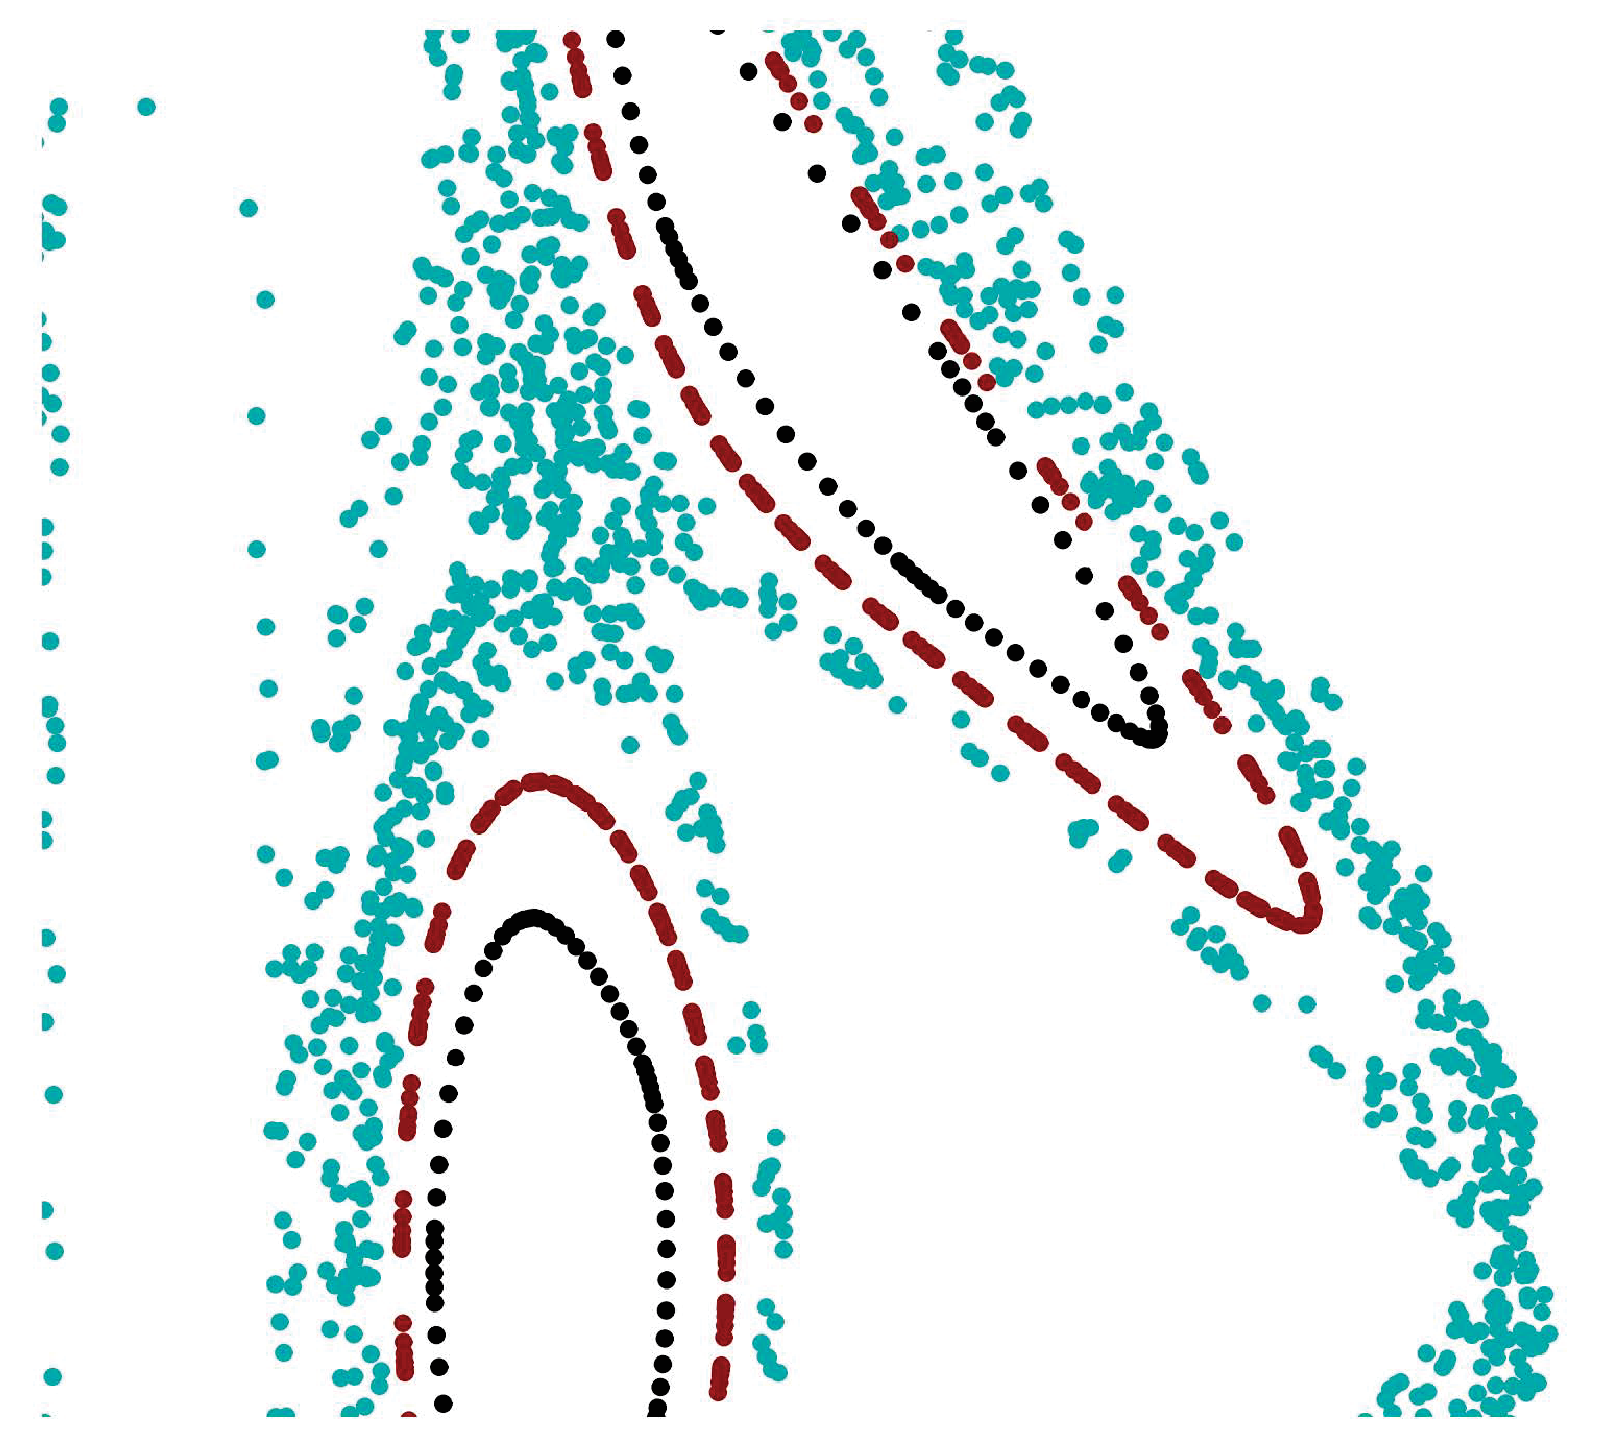
\includegraphics[height=10.cm, angle=0]{nonergodic.eps}
\caption{
KAM tori and nonergodic motion. This is a (Poincar\'e) cross-section of Earth's motion in the three-body problem, with Jupiter's mass set at almost $70$ times its actual value. The closed loops correspond to trajectories that form tori in phase space, whose cross-sections look like deformed circles in our view. The complex filled region is a single trajectory exhibiting chaotic motion, and represents an ergodic component. The tori, each an ergodic component, can together be shown to occupy nonzero volume in phase space, for small Jovian masses. Note that this system is not ergodic according to either of our definitions. The trajectories on the tori never explore the rest of the energy surface. The region $R$ formed by the chaotic domain is invariant under the time evolution; it has positive volume and the region outside $R$ also has positive volume.
}
\label{fig:nonergodic}
\end{figure*}
%===========================================================================================================================

\begin{tcolorbox}[colback=green!5,colframe=green!40!black,title= Definition 1]
In an ergodic system, the trajectory of almost every\footnote{What does almost every mean? Technically, it means all but a set of zero volume (measure zero). Basically, the qualification `almost' is there to avoid problems with unusual, specific initial conditions like all the particles moving precisely at the same velocity in neat rows.} point in phase space eventually passes arbitrarily close\footnote{Why not just assume that every point on the energy surface gets passed through? Boltzmann originally did assume this. However, it can be shown that a smooth curve (our time trajectory) cannot fill up a whole volume (the energy surface). In an ergodic system the trajectory covers the energy surface densely, but not completely.} to every other point (position and momentum) on the surface of constant energy.
\end{tcolorbox}

The most important consequence of ergodicity is that time averages are equal to microcanonical averages\footnote{If an ergodic system equilibrates (i.e., does not oscillate forever), the time average behavior will be determined by the equilibrium behavior; ergodicity then implies that the equilibrium properties are equal to the microcanonical averages.}. Intuitively, since the trajectory $(\mathbb P(t), \mathbb Q(t))$ covers the whole energy surface, the average of any property $O(\mathbb P(t), \mathbb Q(t))$ over time is the same as the average of $O$ over the energy surface. 

The energy surface cannot be divided into components which do not intermingle. Define an ergodic component $R$ of a set $S$\footnote{$S$ is the energy surface.} to be a subset that remains invariant under the flow (so $r(t) \in R$ for all $r(0) \in R$).

\begin{tcolorbox}[colback=green!5,colframe=green!40!black,title= Definition 2]
A time evolution in a set $S$ is ergodic if and only if all the ergodic components $R$ in $S$ either have zero volume or have a volume equal to the volume of $S$.
\end{tcolorbox}
A trajectory $r(t)$ must lie within a single ergodic component. If $r(t)$ covers the energy surface densely, then there is ‘no more room’ for a second ergodic component with non-zero volume. Conversely, if there is only one ergodic component $R$ with volume equal to $S$, then any trajectory starting in $R$ must get arbitrarily close to all points in $R$, otherwise the points in $R$ `far' from the trajectory (outside the closure of the trajectory) would be an invariant set of nonzero volume.

The time averages must equal microcanonical averages. Denote the microcanonical average of an observable $O$ as $\langle O\rangle_S$, and the time average starting at initial condition $(\mathbb P, \mathbb Q)$ as $\overline{O(\mathbb P(0), \mathbb Q(0))} = \lim\limits_{T \rightarrow \infty} (1/T ) \int\limits_0^T O(\mathbb P(t), \mathbb  Q(t)) \dif t$.

The time average $\overline{O}$ equals the ensemble average $\langle O\rangle_S$ for an ergodic system. 

Time averages are constant on trajectories. If $O$ is a nice function (e.g. without any infinities on the energy surface), then
\begin{equation}
\overline{O(\mathbb P(0), \mathbb Q(0))} = \overline{O(\mathbb P(t), \mathbb Q(t))} ~,
\end{equation}
the future time average does not depend on the values of $O$ during the finite time interval $(0, t)$. Thus the time average $\overline{O}$ is constant along the trajectory.\footnote{If we could show that $\overline{O}$ had to be a continuous function, we would now be able to use the first definition of ergodicity to show that it was constant on the energy surface, since our trajectory comes close to every point on the surface. But it is not obvious that $\overline{O}$ is continuous; for example, it
is not continuous for Hamiltonian systems that are not ergodic. Consider two initial conditions at nearby points, one just inside a chaotic region and the other on a KAM torus. The infinite time averages on these two trajectories for most quantities will be quite different; $\overline{O}$ will typically have a jump at the boundary.}

Time averages are constant on the energy surface. Now consider the subset $R_a$ of the energy surface where $\overline{O} < a$, for some value a. Since $\overline{O}$ is constant along a trajectory, any point in $R_a$ is sent under the time evolution to another point in $R_a$, so $R_a$ is an ergodic component. If we have ergodic dynamics on the energy surface, that means the set  $R_a$ has either zero volume or the volume of the energy surface. This implies that $\overline{O}$ is a constant on the energy surface (except on a set of zero volume); its value is $a^\ast$, the lowest value where $R_{a^\ast}$ has the whole volume. Thus the equilibrium, time average value of our observable $O$ is independent of initial condition. 


Time averages equal microcanonical averages. Is this equilibrium value given by the microcanonical ensemble average over S? We need to show that the trajectories do not linger in some regions of the energy surface more than they should (based on the thickness of the energy shell). Liouville's theorem told us that the microcanonical ensemble was time independent, so the
ensemble average equals its time average, which equals the ensemble average of the time average. But the time average is constant (except on a set of zero volume), so in an ergodic system the ensemble average equals the time average everywhere (except on a set of zero volume).\footnote{$\langle O\rangle_S = \langle O(t) \rangle_S = \langle O(\mathbb P(t), \mathbb Q(t))\rangle_S$, where the average $\langle \cdot \rangle_S$ integrates over initial conditions $(\mathbb P(0), \mathbb Q(0))$ but evaluates $O$ at $(\mathbb P(t), \mathbb Q(t))$. Averaging over all time, and using the fact that the time average $\overline{O} = a^\ast$ (almost everywhere), 
\begin{align}
\nonumber \langle O\rangle_S &= \lim\limits_{T\rightarrow \infty} \dfrac{1}{T} \int_0^T \langle O(\mathbb P(t), \mathbb Q(t))\rangle_S \dif t \\
\nonumber &= \left\langle \lim\limits_{T\rightarrow \infty} \dfrac{1}{T} \int_0^T  O(\mathbb P(t), \mathbb Q(t)) \dif t \right\rangle_S \\
\nonumber &= \langle \overline{ O(\mathbb P, \mathbb Q) }\rangle_S = \langle a^\ast \rangle_S = a^\ast ~.
\end{align}
}

















Ergodicity has been proven for the collisions of hard spheres, and for geodesic motion on finite surfaces with constant negative curvature\footnote{Geodesic motion on a sphere would be motion at a constant speed around great circles. Geodesics are the shortest paths between two points. In general relativity, falling bodies travel on geodesics in space–time.}, but not for many systems of immediate practical importance. Indeed, several fundamental problems precisely involve systems which are not ergodic.

















%%%%%%%%%%%%%%%%%%%%%%%%%%%%%%%%%%%%%%%%%%%%%%%%%%%%%%%%%%%%%%%%%%%%%%
\bibliographystyle{unsrt_update}
\bibliography{ref}
%%%%%%%%%%%%%%%%%%%%%%%%%%%%%%%%%%%%%%%%%%%%%%%%%%%%%%%%%%%%%%%%%%%%%%



\end{document}